\documentclass{standalone}
\usepackage{tikz}
\usepackage{float}
\usepackage{amsmath}
\usepackage{lmodern}
\usepackage{amssymb}
\usetikzlibrary{calc}
\usetikzlibrary{hobby}
\usepackage{nicefrac}
\usetikzlibrary{decorations.markings}
\usetikzlibrary{patterns, patterns.meta}
\usetikzlibrary{shapes}
\usetikzlibrary{shapes.misc}
\usepackage{pgfplots}
\pgfplotsset{compat=1.18}
\begin{document}
\centering

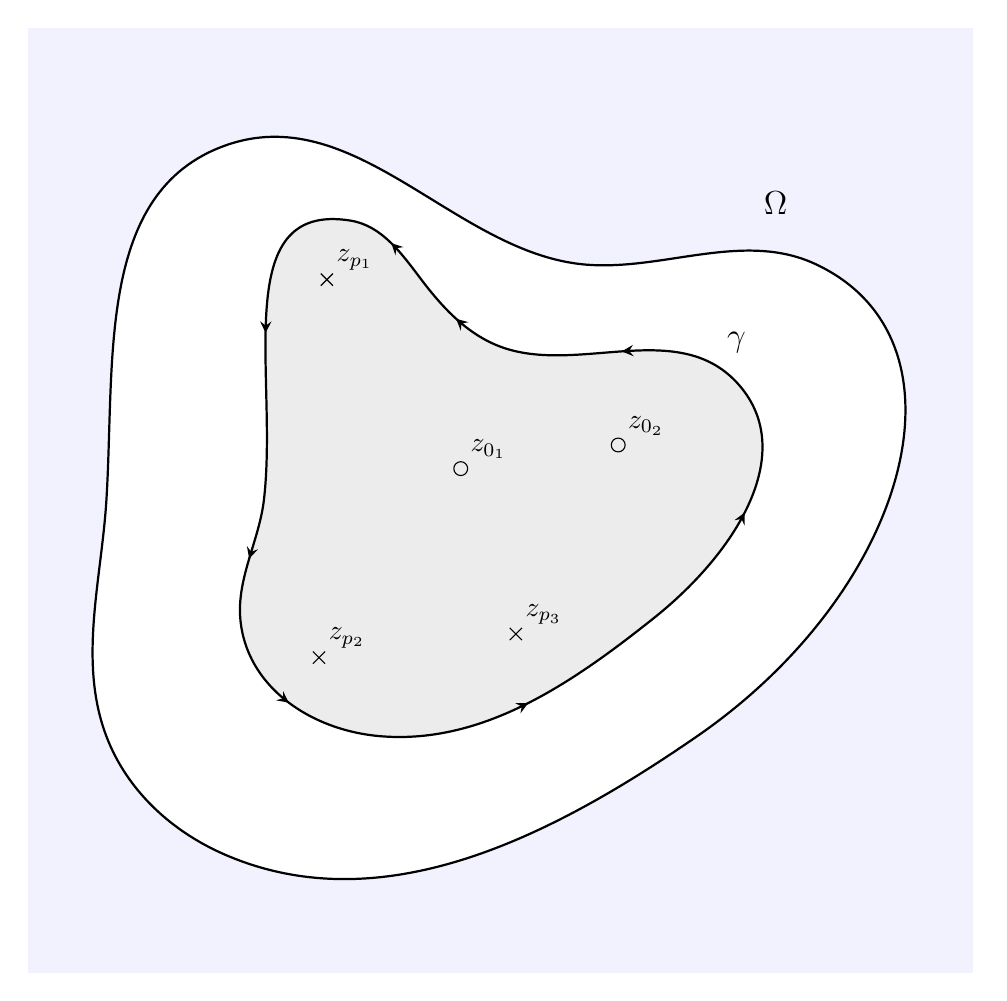
\begin{tikzpicture}

    % define the colors
    \colorlet{GrayBackground}{gray!15}
    \colorlet{BlueBackground}{blue!5}
    % Background for entire canvas
    \colorlet{BlueBackground}{blue!5}

    % Background for entire canvas
    \fill[BlueBackground] (-6,-6) rectangle (6,6);
    \tikzset{
      BigTextFont/.style={font=\large},
      Pole/.style={solid, cross out, minimum size=4pt, inner sep=0pt, draw=black},   % define style for poles=cross
      Zero/.style={solid, circle, minimum size=5pt, inner sep=0pt, draw=black}      % define style for zeroes=cross
    }

    % style to apply some styles to each segment of a path
    \tikzset{on each segment/.style={
      decorate,
      decoration={
        show path construction,
        moveto code={},
        lineto code={
          \path [#1]
          (\tikzinputsegmentfirst) -- (\tikzinputsegmentlast);
        },
        curveto code={
          \path [#1] (\tikzinputsegmentfirst)
          .. controls
          (\tikzinputsegmentsupporta) and (\tikzinputsegmentsupportb)
          ..
          (\tikzinputsegmentlast);
        },
        closepath code={
          \path [#1]
          (\tikzinputsegmentfirst) -- (\tikzinputsegmentlast);
        },
      },
    },
    % style to add an arrow in the middle of a path
    mid arrow/.style={postaction={decorate,decoration={
          markings,
          mark=at position .5 with {\arrow[#1]{stealth}}
        }}},
  }

    %% Macros for drawing poles and zeros

    \newcommand{\DrawPole}[2]{%
    %function for drawing poles
    % #Inputs
    % #1 = coordinate (can be polar like 71.6:1.58)
    % #2 = label (e.g., $z_1$)
    \node[Pole] at (#1) {};
    \node[above right] at (#1) {#2};
    }

    \newcommand{\DrawZero}[2]{%
    %function for drawing poles
    % #Inputs
    % #1 = coordinate (can be polar like 71.6:1.58)
    % #2 = label (e.g., $z_1$)
    \node[Zero] at (#1) {};
    \node[above right] at (#1) {#2};
    }

    %% DEFINE DIFFERENT AREAS
    % define omega space
    \coordinate (OmegaA) at (2.5,-3);
    \coordinate (OmegaB) at (-3.5,-4.5);
    \coordinate (OmegaC) at (-5,-3);
    \coordinate (OmegaD) at (-5,0);
    \coordinate (OmegaE) at (-3.5,4.5);
    \coordinate (OmegaF) at (1,3);
    \coordinate (OmegaG) at (4,3);

    % define contour around poles
    \coordinate (ContourA) at (3,1.5);
    \coordinate (ContourB) at (0,1.95);
    \coordinate (ContourC) at (-1,2.8);
    \coordinate (ContourD) at (-1.9,3.55);
    \coordinate (ContourE) at (-3,0);
    \coordinate (ContourF) at (-3.3,-1.5);
    \coordinate (ContourG) at (-1.5,-3);
    \coordinate (ContourH) at (1.95,-1.5);


    %% FILL AND DRAW THE AREAS

    % draw omega space
    \path [draw=black,thick, fill=white] (OmegaA) to[closed, curve through =
    { (OmegaB) (OmegaC) (OmegaD) (OmegaE) (OmegaF) }] (OmegaG);
    \draw[color=black] (3.5,3.5) node[above, BigTextFont] {$\Omega$};

    % draw contour around poles
    \path [draw=black,thick,postaction={on each segment={mid arrow=black}}, fill=GrayBackground]
    (ContourA) to[closed, curve through =
    { (ContourB) (ContourC) (ContourD) (ContourE) (ContourF) (ContourG) }] (ContourH);
    \node[BigTextFont] at (3,2) {$\mathcal{\gamma}$};

    %% DRAW ZEROES AND POLES
    % draw zeros
    \coordinate (ZeroA) at (-0.5,0.4) {};
    \DrawZero{ZeroA}{$z_{0_1}$}

    \coordinate (ZeroB) at (1.5,0.7);
    \DrawZero{ZeroB}{$z_{0_2}$}
    
    %draw poles
    \coordinate (PoleA) at (-2.2,2.8);
    \DrawPole{PoleA}{$z_{p_1}$}
    
    \coordinate (PoleB) at (-2.3,-2.0);
    \DrawPole{PoleB}{$z_{p_2}$};

    \coordinate (PoleC) at (0.2,-1.7);
    \DrawPole{PoleC}{$z_{p_3}$};

    


\end{tikzpicture}

\end{document}
